\subsection{Integrals in the Plane}
\subsubsection{Vector Fields}
A vector field can be defined as $\vec{F}=\brangle{P(x,y),Q(x,y)}$ where every point $(x,y)$ maps to a corresponding vector.\\
Ex: $\vec{F}=\brangle{x,y}$\\
\centerline{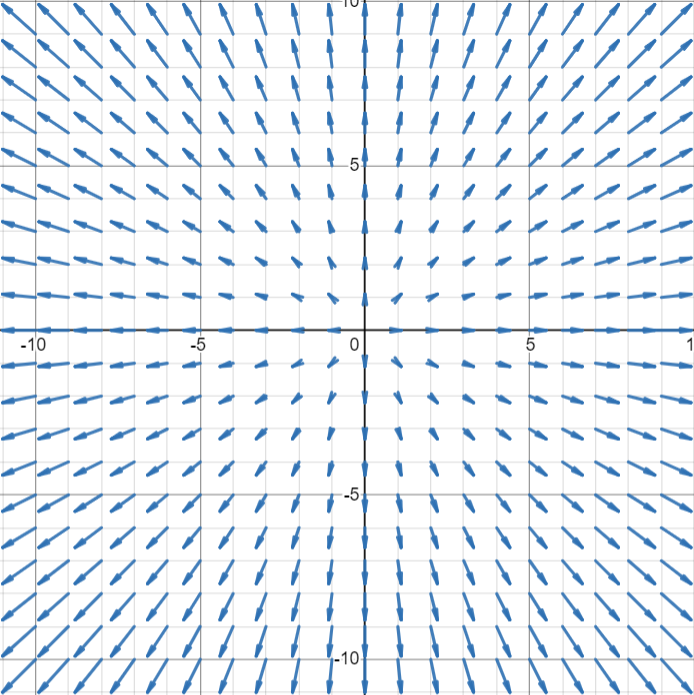
\includegraphics[scale=0.6]{Images/Math217Pictures/vectorFieldEx1.png}}
Ex2: $\vec{F}=\brangle{-y,x}$\\
\centerline{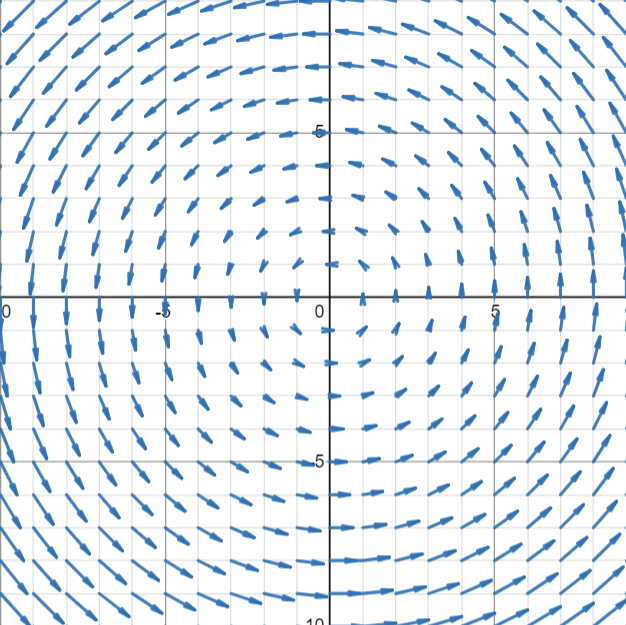
\includegraphics[scale=0.6]{Images/Math217Pictures/vectorFieldEx2.png}}
A vector field is defined to be conservative if it can be represented as the gradient of a function
$$\vec{F}=\nabla f$$
Ex: Conservation of energy:
\begin{align*}
    &\vec{F}=m\vec{a}\\
    &\nabla f=m\frac{d\vec{v}}{dt}\\
    &m\vec{v}\cdot\frac{d\vec{v}}{dt}=\vec{v}\cdot\nabla f\\
    &\brangle{\frac{dx}{dt},\frac{dy}{dt},\frac{dz}{dt}}\cdot\brangle{f_x,f_y,f_z}=\frac{1}{2}m\frac{d}{dt}(\vec{v}\cdot\vec{v})\\
    &\frac{\partial f}{\partial x}\cdot\frac{dx}{dt}+\frac{\partial f}{\partial y}\cdot\frac{dy}{dt}+\frac{\partial f}{\partial z}\cdot\frac{dz}{dt}=\frac{d}{dt}\brround{\frac{1}{2}m\|v\|^2}\\
    &\frac{d}{dt}\brround{\frac{1}{2}mv^2-f(x,y,z)}=0
\end{align*}
A vector field is conservative if the curl is zero and the domain is simply connected (meaning it is continuous and defined everywhere in question).\\
$$\text{curl}(\vec{F})=\nabla\times\vec{F}=\detmatrix{\hat{i}&\hat{j}&\hat{k}\\\frac{\partial}{\partial x}&\frac{\partial}{\partial y}&\frac{\partial}{\partial z}\\P&Q&R}$$
Note that just a curl of $\vec{0}$ is not enough to determine if a vector field is conservative (we will see an example of this later).\\
\\
\textbf{Divergence and Curl}\\
There are two new operations that can be performed on a vector field. These are divergence and curl.\\
If we think of a vector filed as a fluid flow, divergence determines how compressible a vector field is. If there is more fluid being created then destroyed in a region, the divergence in that region will be positive (think of a source of a sink). Similarly, if there is more fluid being destroyed then the divergence will be negative (think of a drain of a sink). A divergence of 0 implies that the fluid is incompressible. The restult of the divergence will be a scalar and it is analogous to the dot product.
$$\text{div}(\vec{F})=\nabla\cdot\vec{F}=P_x+Q_y+R_z$$
Curl is a measure of how non-conservative a vector field is. A curl of zero implies that that a vector field is irrotational.\\
Some notes on divergence and curl.
\begin{itemize}
    \item The image of the gradient are conservative vector fields
    \item The kernal (null space) of curl is the irrotational vector field
    \item If the domain is simply connected then the kernel of curl is equal to the image of the gradient.
    \item When a vector filed is divergence free, every surface is a boundary of a solid.
\end{itemize}
There are many different product rules that relate to divergence and curl. Here is an example:
\begin{align*}
    \nabla\cdot(f\vec{F})&=\nabla\cdot\brangle{fP,fQ,fR}\\
    &=(fP)_x+(fQ)_y+(fR)_z\\
    &=f_xP+f_yQ+f_zR+fP_x+fQ_y+fR_z\\
    &=\brangle{f_x,f_y,f_z}\cdot\brangle{P,Q,R}+f\brangle{P_x,Q_y,R_z}\\
    \nabla\cdot(f\vec{F})&=(\nabla f)\cdot\vec{F}+f(\nabla\cdot\vec{F})
\end{align*}
Ex: Compute $\nabla\cdot(r^k\vec{r})$ for where $\vec{r}=\brangle{x,y,z}$ and $r=\|\vec{r}\|=\sqrt{x^2+y^2+z^2}$
\begin{align*}
    &\nabla\cdot(r^k\vec{r})=(\nabla r^k)\cdot\vec{r}+r^k\nabla\cdot\vec{r}\\
    &\nabla\cdot\vec{r}=\nabla\cdot\brangle{x,y,z}=1+1+1=3\\
    &\nabla r^k=kr^{k-1}\nabla r,\ \nabla r=\brangle{\frac{x}{\sqrt{x^2+y^2+z^2}},\frac{y}{\sqrt{x^2+y^2+z^2}},\frac{z}{\sqrt{x^2+y^2+z^2}}}=\frac{\vec{r}}{r}\\
    &\nabla r^k=kr^{k-2}\vec{r}\\
    &\nabla\cdot(r^k\vec{r})=kr^{k-2}\vec{r}\cdot\vec{r}+3r^k=kr^{k-2}\|\vec{r}\|^2+3r^k\\
    &=(3+k)r^k
\end{align*}
\subsubsection{Line Integrals}
Line integrals over some path $C$ can be computed the same way as with arc length. We first find a parameterization for $C$ and then compute using the following formula,
$$\int_C fds=\int_{t=a}^b f(\vec{r}(t))\|\vec{r}'(t)\|dt$$
Ex: Integrate $f(x,y)=xy^4$ along the right half of the circle $x^2+y^2=16$\\
\begin{align*}
    &C:\ \vec{r}(t)=\brangle{4\cos t,4\sin t},\ -\frac{\pi}{2}\leq t\leq \frac{\pi}{2}\\
    &\vec{r}'(t)=\brangle{-4\sin t,4\cos t}\\
    &\|\vec{r}'(t)\|=\sqrt{16\sin^2t+16\cos^2t}=4\\
    &\int_C fds=\int_{-\pi/2}^{\pi/2}(4\cos t)(4\sin t)^4(4)dt=4^6\brsquare{\frac{\sin^5t}{5}}_{-\pi/2}^{\pi/2}=\frac{8192}{5}
\end{align*}
\subsubsection{Work Integrals}
We can define a path integral inside a force field using the concept of work. Work is the force of the vector field times the distance travelled in the same direction. So we can define an infinitesimal amount of work to be $dW=\vec{F}\cdot d\vec{r}$ which gives the integral formula
$$W=\int_C\vec{F}\cdot d\vec{r}=\int_C(\vec{F}\cdot\hat{T})ds=\int_{t=a}^b\vec{F}(\vec{r}(t))\cdot\vec{r}'(t)dt$$
Note that the shorthand notation $d\vec{r}=\|\vec{r}'(t)\|dt$.\\
Ex: Find $\int_C\vec{F}\cdot d\vec{r}$ where $\vec{F}=\brangle{x,x}$ and $C$ is the curve $3x=y^2$ starting at $(0,0)$ and ending at $(3,3)$.
\begin{align*}
    &\vec{r}(t)=\brangle{\frac{t^2}{3},t}\\
    &\vec{r}'(t)=\brangle{\frac{2}{3}t,1}\\
    &\int_C\vec{F}\cdot d\vec{r}=\int_0^3\brangle{\frac{t^2}{3},\frac{t^2}{3}}\cdot\brangle{\frac{2}{3}t,1}dt=\int_0^3\brround{\frac{2}{9}t^3+\frac{t^2}{3}}dt=\brsquare{\frac{t^4}{18}+\frac{t^3}{9}}_0^3=\frac{15}{2}
\end{align*}
Fundamental Theorem of Line Integrals:\\
This states that if $\vec{F}$ is conservative ($\vec{F}=\nabla f$) then
$$\int_C\vec{F}\cdot d\vec{r}=f(P_2)-f(P_1)$$
meaning that the work integral is path independent.\\
Note that this formula implies that the integral of any closed loop over a conservative vector field is always 0.
$$\oint_C\vec{F}\cdot d\vec{r}=0$$
$\vec{F}$ is conservative when the curl is zero and the domain is simply connected.\\
Ex2: Find $\int_C\vec{F}\cdot d\vec{r}$ where $\vec{F}=\brangle{e^{-x^2}+3y^3-3x^2y,\arctan(y^3)+6xy^2-x^3}$ and $C$ is the closed loop formed by the unit circle in the clockwise direction.
\begin{align*}
    &\nabla\times\vec{F}=\brround{6y^2-3x^2-9y^2+6x^2}\hat{k}=-3y^2\hat{k}\\
    &\text{we can break this up into two different focre fields $\vec{F}_1$ and $\vec{F}_2$}\\
    &\vec{F}_1=\brangle{e^{-x^2}+2y^3-3x^2y,\arctan(y^3)+6xy^2-x^3},\ \nabla\times\vec{F}_1=\vec{0}\\
    &\vec{F}_2=\brangle{y^3,0}\\
    &\vec{F}_1\text{ is conservative so }\int_C\vec{F}_1\cdot d\vec{r}=0\\
    &\int_C\vec{F}_2\cdot d\vec{r}\text{ will require a parameterization}\\
    &\vec{r}(t)=\brangle{-\cos t,\sin t}\\
    &\vec{r}'(t)=\brangle{\sin t,\cos t}\\
    &\int_C\vec{F}_2\cdot\ d\vec{r}=\int_0^{2\pi}\brangle{\sin^3 t,0}\cdot\brangle{\sin t,\cos t}dt=\int_0^{2\pi}\sin^4 tdt=\frac{3\pi}{4}\\
    &\int_C\vec{F}\cdot d\vec{r}=\int_C\vec{F}_1\cdot d\vec{r}+\int_C\vec{F}_2\cdot d\vec{r}=\frac{3\pi}{4}
\end{align*}
Ex3: Find $\int_C\vec{F}\cdot d\vec{r}$ where $\vec{F}=\brangle{\frac{-y}{x^2+y^2},\frac{x}{x^2+y^2}}$ and $C$ is the counterclockwise circle of radius $R$ around the origin.
\begin{align*}
    &\nabla\times\vec{F}=\vec{0}\\
    &\text{$\vec{F}$ is undefined at $(0,0)$, meaning it is not simply connected}\\
    &\text{This means we cannot apply the fundamental theorem of line integrals}\\
    &\vec{r}(t)=\brangle{R\cos t,R\sin t}\\
    &\vec{r}'(t)=\brangle{-R\sin t,R\cos t}\\
    &\int_C\vec{F}\cdot d\vec{r}=\int_0^{2\pi}\brangle{\frac{-R\sin t}{R^2},\frac{R\cos t}{R^2}}\cdot\brangle{-R\sin t,R\cos t}dt=\int_0^{2\pi}(\sin^2t+\cos^2t)dt=2\pi
\end{align*}
\subsubsection{Green's Theorem}
Green's Theorem is an extention of the fundamental theorem of line integrals for closed path integrals. Essentially, it transforms a line integral into a double integral over the enclosed region.\\
For a vector field $\vec{F}=\brangle{P,Q}$
$$\oint_{\partial R}\vec{F}\cdot d\vec{r}=\iint_R(Q_x-P_y)dA$$
Some caveats to this is that the vector field must be defined over the entire region and that the loop travels counterclockwise (it can go counterclockwise but with a change of sign) so that the region will always be to the left of the direction of travel along the loop.\\
We can see this using some previous examples:\\
Ex: Find $\int_C\vec{F}\cdot d\vec{r}$ where $\vec{F}=\brangle{e^{-x^2}+3y^3-3x^2y,\arctan(y^3)+6xy^2-x^3}$ and $C$ is the closed loop formed by the unit circle in the clockwise direction.
\begin{align*}
    &Q_x-P_y=\brround{6y^2-3x^2-9y^2+6x^2}=-3y^2\\
    &\oint_C\vec{F}\cdot d\vec{r}=-\iint_{x^2+y^2=1}-3y^2dA=\int_{\theta=0}^{2\pi}\int_{r=0}^13r^3\sin^2\theta drd\theta\\
    &=\frac{3\pi}{4}
\end{align*}
If a loop is not closed or has a hole in it, we can add another line integral to close the loop so that we can compute with Green's Theorem.\\
Ex2: Find $\int_C\vec{F}\cdot d\vec{r}$ where $\vec{F}=\brangle{\frac{-y}{x^2+y^2},\frac{x}{x^2+y^2}}$ and $C$ is the counterclockwise circle of radius $R$ around the origin.\\
Notice with this vector field the center is undefined so we can create another infinitesimally small loop around the origin so that the vector field is now defined everywhere.
\begin{align*}
    &C'=\brcurly{x^2+y^2=\epsilon^2,\ |\epsilon|\ll1}\text{ travelling clockwise}\\
    &\oint_{\partial R}\vec{F}\cdot d\vec{r}=\int_C\vec{F}\cdot d\vec{r}+\int_{C'}\vec{F}\cdot d\vec{r}\\
    &Q_x-P_y=0\\
    &\oint_{\partial R}\vec{F}\cdot d\vec{r}=\iint 0 d\vec{r}=0\\
    &\vec{r}=\brangle{-\epsilon\cos t,\epsilon\sin t}\\
    &\vec{r}'=\brangle{\epsilon\sin t,\epsilon\cos t}\\
    &\int_{C'}\vec{F}\cdot d\vec{r}=\lim_{\epsilon\to0}\int_0^{2\pi}\brangle{\frac{-\epsilon\sin t}{\epsilon^2},\frac{\epsilon\cos t}{\epsilon^2}}\cdot\brangle{-\epsilon\sin t,\epsilon\cos t}=2\pi\\
    &\Ra \int_C\vec{F}\cdot d\vec{r}=\oint_{\partial R}\vec{F}\cdot d\vec{r}-\int_{C'}\vec{F}\cdot d\vec{r}=2\pi
\end{align*}
Ex3: Find the area of the ellipse $\frac{x^2}{a^2}+\frac{y^2}{b^2}=1$
\begin{align*}
    &\text{need }Q_x-P_y=1\\
    &\vec{F}=\brangle{-\frac{y}{2},\frac{x}{2}}\\
    &\vec{r}=\brangle{a\cos t,b\sin t}\\
    &\vec{r}'=\brangle{-a\sin t,b\cos t}\\
    &\oint\vec{F}\cdot d\vec{r}=\int_0^{2\pi}\frac{1}{2}\brangle{-b\sin t,a\cos t}\cdot\brangle{-a\sin t,b\cos t}dt=\frac{1}{2}\int_0^{2\pi}(ab\sin^2t+ab\cos^2t)dt\\
    &=\frac{ab}{2}\int_0^{2\pi}dt=\pi ab
\end{align*}